\documentclass{article}
% generated by Madoko, version 1.0.0-rc6
%mdk-data-line={1}


\usepackage[heading-base={2},section-num={False},bib-label={True}]{madoko2}


\begin{document}



\mdhr{}%mdk

\noindent title: 博客诞生季
categories: 随笔
date: 2016-04-17 11:25:32%mdk

\subsection{0.1.\hspace*{0.5em}tags: Hexo}\label{sec-tags--hexo}%mdk%mdk

\section{1.\hspace*{0.5em}前言}\label{section}%mdk%mdk

\noindent折腾了两天,终于把期待很久的博客弄上线了,这就如同上了电视一般激动,所以激动的同时,也记录一下这个
艰辛的过程,留给自己,帮助他人。%mdk

\section{2.\hspace*{0.5em}Hexo}\label{sec-hexo}%mdk%mdk

\noindent Hexo的作者是tommy351,根据官方介绍,Hexo是一个简单、快速、强大的博客发布工具,支持Markdown格式%mdk

\subsection{2.1.\hspace*{0.5em}安装}\label{section}%mdk%mdk

\noindent打开git%mdk
\begin{mdpre}%mdk
\noindent npm~install~-g~hexo%mdk
\end{mdpre}
\subsection{2.2.\hspace*{0.5em}初始化}\label{section}%mdk%mdk

\noindent在我的电脑中建立一个名字叫「Hexo」的文件夹,然后在此文件夹中右键打开Git Bash%mdk
\begin{mdpre}%mdk
\noindent hexo~init%mdk
\end{mdpre}\noindent初始化完 \emph{cd} 进你初始化化的目录

\subsection{2.3.\hspace*{0.5em}生成静态页面}\label{section}%mdk%mdk

\noindent以下命令会在你 \emph{init} 目录下生成一个public文件夹%mdk
\begin{mdpre}%mdk
\noindent hexo~generate%mdk
\end{mdpre}\noindent如果是第二次生成,那要执行以下命令进行清除public文件夹
\begin{mdpre}%mdk
\noindent hexo~clean\\
%mdk
\end{mdpre}
\subsection{2.4.\hspace*{0.5em}本地启动}\label{section}%mdk%mdk
\begin{mdpre}%mdk
\noindent hexo~server\\
%mdk
\end{mdpre}\noindent执行完成后,浏览器输入\href{http://localhost:4000}{http://localhost:4000}就可以看到效果

\subsection{2.5.\hspace*{0.5em}写文章}\label{section}%mdk%mdk

\noindent执行new命令,生成指定名称的文章至hexo\textbackslash{}source\_posts\textbackslash{}postName.md%mdk
\begin{mdpre}%mdk
\noindent hexo~new~page~"postName"~\#新建文章~~~~%mdk
\end{mdpre}
\subsection{2.6.\hspace*{0.5em}文章摘要}\label{section}%mdk%mdk

\noindent在需要显示摘要的地方添加以下代码即可%mdk
\begin{mdpre}%mdk
\noindent以上是摘要\\
\textless{}!--more--\textgreater{}\\
以下是余下全文\\
%mdk
\end{mdpre}
\subsection{2.7.\hspace*{0.5em}新建页面}\label{section}%mdk%mdk

\noindent执行new命令,生成指定名称的文件夹至hexo\textbackslash{}source\textbackslash{}pageName,并且生成index.md至文件夹%mdk
\begin{mdpre}%mdk
\noindent hexo~new~pageName~\#新建页面\\
%mdk
\end{mdpre}
\subsection{2.8.\hspace*{0.5em}部署Hexo}\label{sec-hexo}%mdk%mdk

\noindent以下命令建立在已成功构建了Github远程端的前提下,这里就不一概述了%mdk
\begin{mdpre}%mdk
\noindent hexo~deloy~\#部署到Github\\
%mdk
\end{mdpre}
\subsection{2.9.\hspace*{0.5em}常用命令}\label{section}%mdk%mdk
\begin{mdpre}%mdk
\noindent hexo~new~"postName"~\#新建文章\\
hexo~new~page~"pageName"~\#新建页面\\
hexo~generate~\#生成静态页面至public目录\\
hexo~server~\#开启预览访问端口(默认端口4000,'ctrl~+~c'关闭server)\\
hexo~deploy~\#将.deploy目录部署到GitHub\\
%mdk
\end{mdpre}\noindent简写
\begin{mdpre}%mdk
\noindent hexo~n~==~hexo~new\\
hexo~g~==~hexo~generate\\
hexo~s~==~hexo~server\\
hexo~d~==~hexo~deploy\\
%mdk
\end{mdpre}
\section{\mdinline{width=}{\href{images/3.png}{3}}.\hspace*{0.5em}主题}\label{section}%mdk%mdk

\noindent搭建hexo时,会给一个初始的主题\textbf{landscape},但是人各有所好,不是每个人都会喜欢
。所以选择一个自己喜欢的主题是很重要的,就像穿衣服一样。%mdk

\subsection{3.1.\hspace*{0.5em}推荐主题}\label{section}%mdk%mdk

\begin{itemize}%mdk

\item{}
pacman: 大气,最重要的是功能齐全%mdk%mdk

\item{}
yilia: 美观,但是有一定的Bug%mdk%mdk

\item{}
next: 现在正在使用,添加插件什么的很方便,很喜欢%mdk%mdk
%mdk
\end{itemize}%mdk

\subsection{3.2.\hspace*{0.5em}Next主题}\label{sec-next}%mdk%mdk

\noindent有很完整的教程,这里就做做搬运工了%mdk

\begin{itemize}%mdk

\item{}
\href{http://theme-next.iissnan.com/getting-started.html}{官方教程}%mdk%mdk

\item{}
\href{https://notes.wanghao.work/2015-10-21-\%25E4\%25B8\%25BANexT\%25E4\%25B8\%25BB\%25E9\%25A2\%2598\%25E6\%25B7\%25BB\%25E5\%258A\%25A0\%25E6\%2596\%2587\%25E7\%25AB\%25A0\%25E9\%2598\%2585\%25E8\%25AF\%25BB\%25E9\%2587\%258F\%25E7\%25BB\%259F\%25E8\%25AE\%25A1\%25E5\%258A\%259F\%25E8\%2583\%25BD.html\%23\%25E9\%2585\%258D\%25E7\%25BD\%25AELeanCloud}{为NexT主题添加文章阅读量统计功能}: 注意后面要加Web安全那一块才能生效%mdk%mdk

\item{}
\href{http://zhiho.github.io/2015/09/29/hexo-next/}{Hexo搭建GitHub博客(三)- NexT主题配置使用}:解惑我很多问题%mdk%mdk
%mdk
\end{itemize}%mdk

\subsection{3.3.\hspace*{0.5em}域名}\label{section}%mdk%mdk

\noindent对于有着情怀的我们来说,怎么可能忍受一直用着\textbf{MyName.github.io}进入我们的博客,所以呢?为了看起来更拉风当然要弄个域名了%mdk

\subsubsection{3.3.1.\hspace*{0.5em}购买域名}\label{section}%mdk%mdk

\paragraph{推荐}\label{section}%mdk%mdk

\begin{itemize}%mdk

\item{}
\href{https://sg.godaddy.com/zh?isc=cjc99com\%26ci=}{Godaddy}: 毕竟是国际大厂商,也支持支付宝%mdk%mdk

\item{}
\href{https://www.aliyun.com/?spm=5176.3047821.1.1.POmfMt}{阿里云}: 支持国产也是很重要的%mdk%mdk
%mdk
\end{itemize}%mdk

\subsubsection{3.3.2.\hspace*{0.5em}DNS服务器}\label{sec-dns}%mdk%mdk

\paragraph{推荐}\label{section}%mdk%mdk

\begin{itemize}[noitemsep,topsep=\mdcompacttopsep]%mdk

\item\href{https://www.dnspod.cn/}{DNSPOO}: 职业DNS服务商%mdk

\item\href{https://www.aliyun.com/?spm=5176.3047821.1.1.POmfMt}{阿里云}: 在阿里云购买的域名,那用他自己的DNS当然最方便,不用更改%mdk
%mdk
\end{itemize}%mdk

\subsubsection{3.3.3.\hspace*{0.5em}域名与Github}\label{sec-github}%mdk%mdk

\noindent因为我用的阿里云的,所以以阿里云的方式作为参考%mdk

\begin{enumerate}[noitemsep,topsep=\mdcompacttopsep]%mdk

\item进入阿里云主页,点击登录
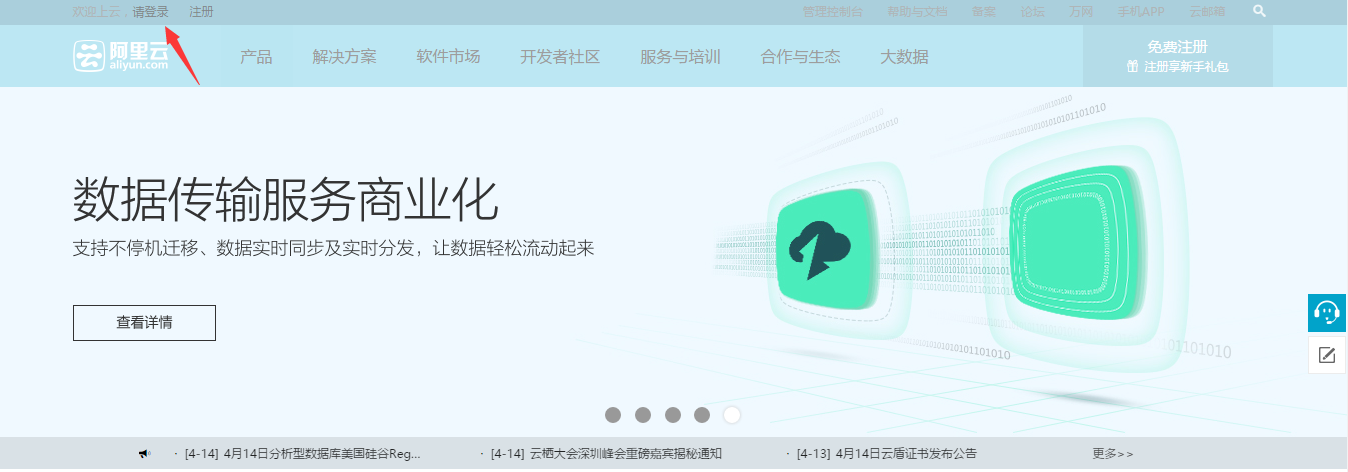
\includegraphics[keepaspectratio=true,width=\dimmin{}{\dimwidth{0.90}}]{images/3}{}%mdk
%mdk
\end{enumerate}%mdk

\begin{enumerate}[noitemsep,topsep=\mdcompacttopsep,start=2]%mdk

\item登陆后,点击万网购买你喜欢并且存在的域名

\includegraphics[keepaspectratio=true,width=\dimmin{}{\dimwidth{0.90}}]{images/4}{}%mdk
%mdk
\end{enumerate}%mdk

\begin{enumerate}[noitemsep,topsep=\mdcompacttopsep,start=3]%mdk

\item{}
购买完成后,进入管理控制台
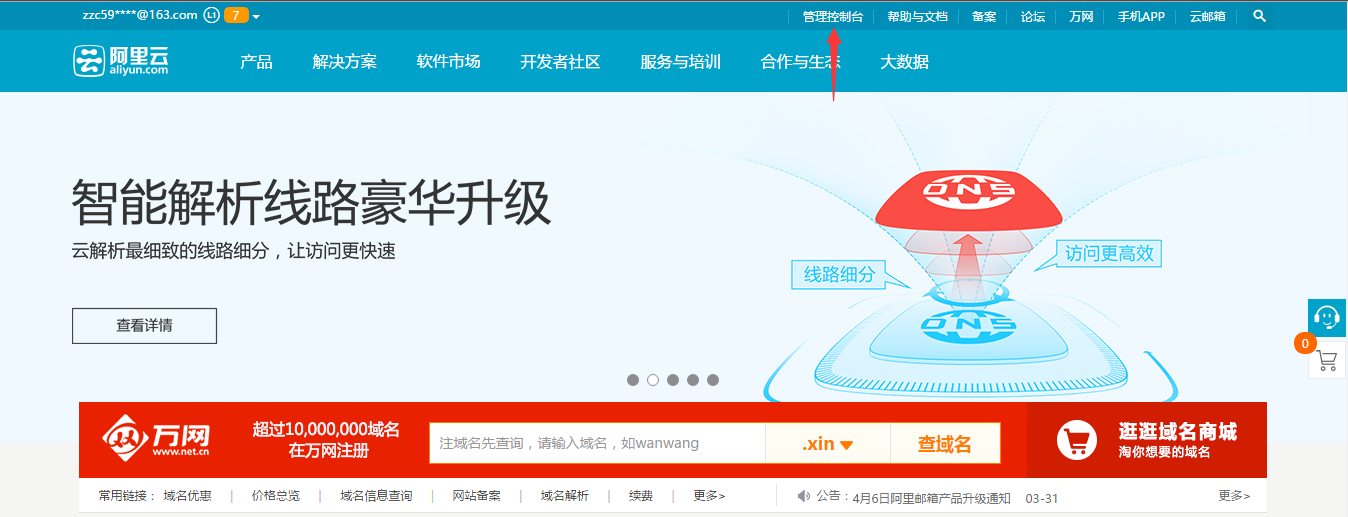
\includegraphics[keepaspectratio=true,width=\dimmin{}{\dimwidth{0.90}}]{images/5}{}%mdk%mdk
%mdk
\end{enumerate}%mdk

\begin{enumerate}[noitemsep,topsep=\mdcompacttopsep,start=4]%mdk

\item点击域名,可以看到域名列表,然后在相应的域名处点击管理
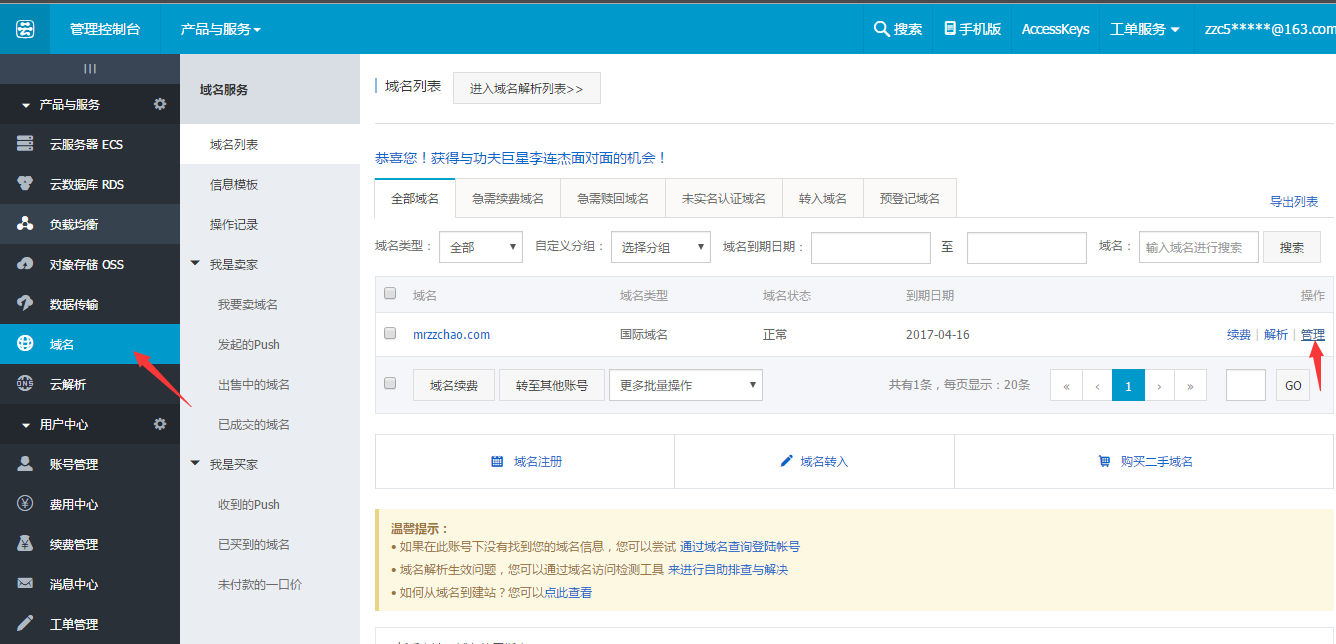
\includegraphics[keepaspectratio=true,width=\dimmin{}{\dimwidth{0.90}}]{images/6}{}%mdk
%mdk
\end{enumerate}%mdk%mdk


\end{document}
